% ─────────────────────────────────────────────────────────────────────────────
% Sec. 4  Experiments. Tables / figures are generated by results/paper/build_paper_results.py
% (re-run it after new results arrive; cells still missing print as a red "?").
% Needs in preamble.tex: \usepackage{multirow} \usepackage{colortbl} \definecolor{oursbg}{HTML}{E8F0FC}
% ─────────────────────────────────────────────────────────────────────────────
\section{Experiments}
\label{sec:exp}

\providecommand{\pend}{\textcolor{red}{?}}

\begin{table*}[t]
  \centering
  \footnotesize
  \setlength{\tabcolsep}{4pt}
  \begin{tabular}{l cc c cc c ccc}
    \toprule
    & \multicolumn{2}{c}{Document} & Real-world & \multicolumn{2}{c}{High resolution} & & \multicolumn{3}{c}{Saving \vs uncompressed$\uparrow$} \\
    \cmidrule(lr){2-3}\cmidrule(lr){4-4}\cmidrule(lr){5-6}\cmidrule(lr){8-10}
    Method & DocVQA & InfoVQA & MME-RW & HR-Bench 4K & V$^*$ Bench & Avg.\ (\%) & TTFT & Memory & FLOPs \\
    \midrule
    \multicolumn{10}{c}{\textit{Upper bound: all visual tokens}} \\
    Uncompressed & 91.4 & 78.7 & 51.6 & 62.0 & 83.8 & 100.0 & 1.0$\times$ & 1.0$\times$ & 1.0$\times$ \\
    \midrule
    \multicolumn{10}{c}{\textit{Budget $B=1536$ visual tokens (default), $\approx$21\% of all visual tokens}} \\
    FastV~\cite{fastv} & 84.0 & 61.0 & 46.9 & \underline{59.0} & 79.1 & 90.0 & & & \\
    & {\scriptsize 91.9\%} & {\scriptsize 77.4\%} & {\scriptsize 90.9\%} & {\scriptsize 95.2\%} & {\scriptsize 94.4\%} & {\scriptsize ($\downarrow$10.0)} & \multirow{-2}{*}{\underline{2.5$\times$}} & \multirow{-2}{*}{1.5$\times$} & \multirow{-2}{*}{\underline{2.9$\times$}} \\
    SparseVLM~\cite{sparsevlm} & 55.1 & 62.2 & \underline{50.2} & \textbf{59.5} & \underline{79.6} & 85.5 & & & \\
    & {\scriptsize 60.3\%} & {\scriptsize 79.1\%} & {\scriptsize 97.4\%} & {\scriptsize 96.0\%} & {\scriptsize 95.0\%} & {\scriptsize ($\downarrow$14.5)} & \multirow{-2}{*}{2.2$\times$} & \multirow{-2}{*}{1.5$\times$} & \multirow{-2}{*}{2.4$\times$} \\
    VisionZip~\cite{visionzip} & 48.7 & 47.6 & 41.7 & 49.0 & 70.2 & 71.5 & & & \\
    & {\scriptsize 53.3\%} & {\scriptsize 60.4\%} & {\scriptsize 80.9\%} & {\scriptsize 79.0\%} & {\scriptsize 83.8\%} & {\scriptsize ($\downarrow$28.5)} & \multirow{-2}{*}{\textbf{2.7$\times$}} & \multirow{-2}{*}{\underline{4.2$\times$}} & \multirow{-2}{*}{\textbf{3.2$\times$}} \\
    IF-Prune~\cite{ifprune} & \textbf{88.2} & \underline{72.7} & 49.3 & 57.5 & \textbf{81.7} & \underline{94.9} & & & \\
    & {\scriptsize 96.5\%} & {\scriptsize 92.3\%} & {\scriptsize 95.6\%} & {\scriptsize 92.7\%} & {\scriptsize 97.5\%} & {\scriptsize ($\downarrow$5.1)} & \multirow{-2}{*}{1.5$\times$} & \multirow{-2}{*}{0.7$\times$} & \multirow{-2}{*}{1.8$\times$} \\
    \rowcolor{oursbg}
    \method (ours) & \underline{87.0}$^{\downarrow}$ & \textbf{74.8}$^{\uparrow}$ & \textbf{52.1}$^{\uparrow}$ & 56.5 & 77.5 & \textbf{95.0} & & & \\
    \rowcolor{oursbg}
    & {\scriptsize 95.2\%} & {\scriptsize 95.0\%} & {\scriptsize 100.9\%} & {\scriptsize 91.1\%} & {\scriptsize 92.5\%} & {\scriptsize ($\downarrow$5.0)} & \multirow{-2}{*}{2.4$\times$} & \multirow{-2}{*}{\textbf{5.0$\times$}} & \multirow{-2}{*}{\textbf{3.2$\times$}} \\
    \midrule
    \multicolumn{10}{c}{\textit{Budget $B=2560$ visual tokens, $\approx$35\% of all visual tokens}} \\
    FastV~\cite{fastv} & \underline{89.6} & 70.5 & 50.1 & \underline{59.0} & \underline{81.7} & 95.5 & & & \\
    & {\scriptsize 98.0\%} & {\scriptsize 89.5\%} & {\scriptsize 97.2\%} & {\scriptsize 95.2\%} & {\scriptsize 97.5\%} & {\scriptsize ($\downarrow$4.5)} & \multirow{-2}{*}{\underline{2.0$\times$}} & \multirow{-2}{*}{1.5$\times$} & \multirow{-2}{*}{\underline{2.2$\times$}} \\
    SparseVLM~\cite{sparsevlm} & 69.8 & 71.1 & \underline{51.8} & 57.0 & 81.2 & 91.2 & & & \\
    & {\scriptsize 76.4\%} & {\scriptsize 90.3\%} & {\scriptsize 100.4\%} & {\scriptsize 91.9\%} & {\scriptsize 96.9\%} & {\scriptsize ($\downarrow$8.8)} & \multirow{-2}{*}{1.7$\times$} & \multirow{-2}{*}{1.4$\times$} & \multirow{-2}{*}{1.8$\times$} \\
    VisionZip~\cite{visionzip} & 62.8 & 57.9 & 45.9 & 57.5 & 76.4 & 83.0 & & & \\
    & {\scriptsize 68.8\%} & {\scriptsize 73.5\%} & {\scriptsize 89.0\%} & {\scriptsize 92.7\%} & {\scriptsize 91.2\%} & {\scriptsize ($\downarrow$17.0)} & \multirow{-2}{*}{\textbf{2.1$\times$}} & \multirow{-2}{*}{\underline{2.8$\times$}} & \multirow{-2}{*}{\textbf{2.4$\times$}} \\
    IF-Prune~\cite{ifprune} & \underline{89.6} & \underline{74.8} & 49.9 & \textbf{59.5} & \textbf{83.8} & \underline{97.1} & & & \\
    & {\scriptsize 98.0\%} & {\scriptsize 95.0\%} & {\scriptsize 96.8\%} & {\scriptsize 96.0\%} & {\scriptsize 100.0\%} & {\scriptsize ($\downarrow$2.9)} & \multirow{-2}{*}{1.3$\times$} & \multirow{-2}{*}{0.7$\times$} & \multirow{-2}{*}{1.5$\times$} \\
    \rowcolor{oursbg}
    \method (ours) & \textbf{90.1} & \textbf{78.6}$^{\uparrow}$ & \textbf{52.2} & 58.0 & 79.6 & \textbf{97.6} & & & \\
    \rowcolor{oursbg}
    & {\scriptsize 98.5\%} & {\scriptsize 99.8\%} & {\scriptsize 101.1\%} & {\scriptsize 93.5\%} & {\scriptsize 95.0\%} & {\scriptsize ($\downarrow$2.4)} & \multirow{-2}{*}{1.7$\times$} & \multirow{-2}{*}{\textbf{3.6$\times$}} & \multirow{-2}{*}{\underline{2.2$\times$}} \\
    \midrule
    \multicolumn{10}{c}{\textit{Budget $B=3072$ visual tokens, $\approx$42\% of all visual tokens}} \\
    FastV~\cite{fastv} & \textbf{90.8} & 73.6 & 49.7 & \textbf{61.0} & \underline{82.7} & 97.2 & & & \\
    & {\scriptsize 99.4\%} & {\scriptsize 93.5\%} & {\scriptsize 96.3\%} & {\scriptsize 98.4\%} & {\scriptsize 98.7\%} & {\scriptsize ($\downarrow$2.8)} & \multirow{-2}{*}{\underline{1.8$\times$}} & \multirow{-2}{*}{1.5$\times$} & \multirow{-2}{*}{\underline{2.0$\times$}} \\
    SparseVLM~\cite{sparsevlm} & 69.8 & 72.5 & \underline{51.0} & 57.0 & \textbf{83.8} & 91.8 & & & \\
    & {\scriptsize 76.3\%} & {\scriptsize 92.1\%} & {\scriptsize 98.8\%} & {\scriptsize 91.9\%} & {\scriptsize 100.0\%} & {\scriptsize ($\downarrow$8.2)} & \multirow{-2}{*}{1.5$\times$} & \multirow{-2}{*}{1.3$\times$} & \multirow{-2}{*}{1.6$\times$} \\
    VisionZip~\cite{visionzip} & 68.8 & 61.8 & 47.4 & 56.5 & 78.5 & 86.1 & & & \\
    & {\scriptsize 75.3\%} & {\scriptsize 78.5\%} & {\scriptsize 91.9\%} & {\scriptsize 91.1\%} & {\scriptsize 93.8\%} & {\scriptsize ($\downarrow$13.9)} & \multirow{-2}{*}{\textbf{1.9$\times$}} & \multirow{-2}{*}{\underline{2.4$\times$}} & \multirow{-2}{*}{\textbf{2.2$\times$}} \\
    IF-Prune~\cite{ifprune} & 90.1 & \underline{75.1} & 49.8 & \textbf{61.0} & 82.2 & \underline{97.4} & & & \\
    & {\scriptsize 98.5\%} & {\scriptsize 95.4\%} & {\scriptsize 96.5\%} & {\scriptsize 98.4\%} & {\scriptsize 98.1\%} & {\scriptsize ($\downarrow$2.6)} & \multirow{-2}{*}{1.2$\times$} & \multirow{-2}{*}{0.7$\times$} & \multirow{-2}{*}{1.4$\times$} \\
    \rowcolor{oursbg}
    \method (ours) & \underline{90.3} & \textbf{79.4}$^{\uparrow}$ & \textbf{53.5}$^{\uparrow}$ & \underline{59.5} & 81.7 & \textbf{99.3} & & & \\
    \rowcolor{oursbg}
    & {\scriptsize 98.8\%} & {\scriptsize 100.8\%} & {\scriptsize 103.6\%} & {\scriptsize 96.0\%} & {\scriptsize 97.5\%} & {\scriptsize ($\downarrow$0.7)} & \multirow{-2}{*}{1.4$\times$} & \multirow{-2}{*}{\textbf{2.7$\times$}} & \multirow{-2}{*}{1.8$\times$} \\
    \bottomrule
  \end{tabular}
  \caption{\textbf{Accuracy and cost on InternVL3.5-8B.} For each method, the first row is the score on each benchmark (ANLS for DocVQA and InfoVQA, CircularEval accuracy for HR-Bench, accuracy otherwise) and the second row is its percentage of the uncompressed model; Avg.\ is the mean percentage over the five benchmarks. HR-Bench 8K is reported separately in \cref{tab:hr8k}. Cost is reported as the saving relative to the uncompressed model (higher is better) in median time to first token, peak memory on top of the model weights, and prefill FLOPs, averaged over the five benchmarks (absolute values in the supplementary material); IF-Prune uses \emph{more} memory than the uncompressed model because of its guide model. $^{\uparrow}$/$^{\downarrow}$: \method is significantly better/worse than the strongest baseline on that benchmark (paired bootstrap, 95\%); unmarked differences are not significant. Best compressed result per budget in \textbf{bold}, second \underline{underlined}.}
  \label{tab:main}
\end{table*}


% ─────────────────────────────────────────────────────────────────────────────
\subsection{Setup}
\label{sec:setup}

\paragraph{Models and benchmarks.}
We evaluate on InternVL3.5-4B, -8B, and -14B~\cite{internvl35}, and use the 8B model unless stated
otherwise. We cover three kinds of high-resolution inputs: documents (DocVQA val~\cite{docvqa}, 5,349
questions; InfoVQA val~\cite{infovqa}, 2,801), real-world scenes (MME-RealWorld Lite~\cite{mmerealworld},
1,919), and very high-resolution images with small targets (HR-Bench 4K and 8K~\cite{hrbench}, 800
questions each; V$^*$ Bench~\cite{vstar}, 191). We report ANLS on DocVQA and InfoVQA, CircularEval
accuracy on HR-Bench (a question counts only if all four option orders are answered correctly), and
multiple-choice accuracy otherwise. All methods use greedy decoding and the same prompts, and start
from the same official dynamic tiling with up to $N_{\max}=47$ tiles plus a thumbnail.

\paragraph{Baselines.}
We compare with FastV~\cite{fastv}, SparseVLM~\cite{sparsevlm}, VisionZip~\cite{visionzip}, and
IF-Prune~\cite{ifprune}, ported to InternVL3.5 from the official code with the official
hyperparameters: FastV and IF-Prune prune at layer 2, IF-Prune uses the released InternVL2.5-1B guide
model, SparseVLM prunes at the official relative depths with its pruning rate calibrated per budget,
and VisionZip keeps dominant and contextual tokens in each tile. For all methods, the budget $B$ is the
number of visual tokens left in the KV cache. Implementation details are in the supplementary material.

\paragraph{Efficiency measurement.}
All measurements use one NVIDIA A6000 (48\,GB), bfloat16, and batch size 1. TTFT is the wall-clock time
to the first generated token, including the vision encoder and any scoring or guide model, and we report the median over 50 images per benchmark after one warm-up image. Memory is the peak
allocated GPU memory minus the model weights; for IF-Prune it includes the guide model. FLOPs count the
vision encoder and the prefill up to the first token.

\paragraph{Protocol.}
All \method hyperparameters are fixed on held-out calibration data (\cref{sec:impl}); no test set is used
for any choice. We test differences with a paired bootstrap over questions (or CircularEval groups) at
95\% confidence.

% ─────────────────────────────────────────────────────────────────────────────
\subsection{Accuracy at a fraction of the cost}
\label{sec:main}

\cref{tab:main} compares all methods at three budgets. At the default budget $B=1536$, which keeps about
a fifth of the visual tokens, \method retains 94.5\% of the uncompressed accuracy on average, on par with
IF-Prune (94.6\%) and well above FastV (90.9\%), SparseVLM (87.1\%), and VisionZip (72.7\%). It does so
at the lowest cost: 0.41\,GB of memory, 7$\times$ less than IF-Prune and 3$\times$ less than FastV and
SparseVLM, and 61\% of the TTFT of IF-Prune. At $B=3072$, \method has the highest average accuracy of
all methods (98.3\%) while still using the least memory.

\method is strongest where the answer depends on the layout of the whole image. On InfoVQA it is
significantly better than every baseline at every budget, by 2.1 to 4.3 points over the strongest one,
and on MME-RealWorld it even exceeds the uncompressed model. On HR-Bench and V$^*$ Bench, which ask about
small objects, \method is within a few points of the best baseline, and none of these differences is
significant at any budget. We analyze this case in \cref{sec:analysis}.

\begin{figure}[t]
  \centering
  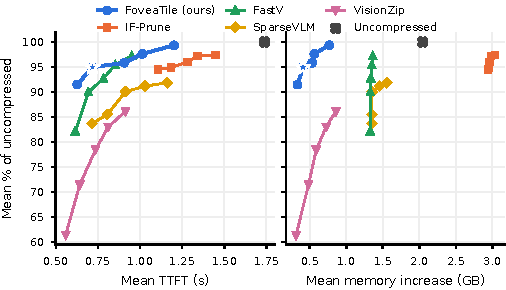
\includegraphics[width=\linewidth]{figures/fig_pareto.pdf}
  \caption{\textbf{Accuracy--cost trade-off} on InternVL3.5-8B, averaged over the six benchmarks, for
  $B\in\{1024,1536,2048,2560,3072\}$. The star marks the default \method budget. \method uses the least
  memory at every budget; in TTFT it shares the frontier with FastV and is faster than IF-Prune at equal
  accuracy.}
  \label{fig:pareto}
\end{figure}

\cref{fig:pareto} shows the full trade-off over five budgets. In memory, \method is the best
curve at every budget: even its largest budget uses less memory than any budget of FastV, SparseVLM,
or IF-Prune. In TTFT, \method and FastV form the frontier: \method is ahead at the lowest and highest
budgets, and FastV between 0.8 and 1.0\,s. \method dominates SparseVLM and IF-Prune, and at about the
same TTFT as IF-Prune at $B=1536$ (1.2\,s) it reaches 98.3\% instead of 94.6\%. The exception is
the smallest budget, $B=1024$, where IF-Prune retains more accuracy (94.3\% \vs 91.7\%) at 1.7$\times$ the
TTFT and 9$\times$ the memory of \method.

% ─────────────────────────────────────────────────────────────────────────────
\subsection{Cost independent of resolution}
\label{sec:scaling}

\begin{figure}[t]
  \centering
  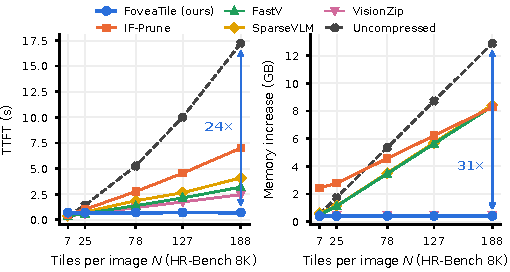
\includegraphics[width=\linewidth]{figures/fig_scaling.pdf}
  \caption{\textbf{Cost as the input resolution grows} (HR-Bench 8K, $B=1536$, tile cap raised so that
  images split into 7 to 188 tiles). \method stays flat at 0.7\,s and 0.4\,GB. VisionZip's memory is also
  flat (its line overlaps ours), but its TTFT grows with $N$ because every tile is encoded.}
  \label{fig:scaling}
\end{figure}

\providecommand{\pend}{\textcolor{red}{?}}

\begin{table}[t]
  \centering
  \footnotesize
  \setlength{\tabcolsep}{3.2pt}
  \begin{tabular}{l ccc ccc}
    \toprule
    & \multicolumn{3}{c}{25 tiles} & \multicolumn{3}{c}{188 tiles} \\
    \cmidrule(lr){2-4}\cmidrule(lr){5-7}
    Method & Acc. & TTFT & Mem. & Acc. & TTFT & Mem. \\
    \midrule
    Uncompressed & 56.5 & 1.44 & 1.79 & 49.0 & 17.22 & 12.90 \\
    \midrule
    FastV & \textbf{54.0} & 0.63 & 1.16 & 42.5 & 3.19 & 8.34 \\
    SparseVLM & 53.5 & 0.76 & 1.18 & \pend & 4.09 & 8.44 \\
    VisionZip & 44.5 & \textbf{0.58} & 0.49 & 27.0 & 2.45 & 0.49 \\
    IF-Prune & 52.5 & 1.04 & 2.81 & \textbf{52.0} & 7.00 & 8.28 \\
    \rowcolor{oursbg}
    \method (ours) & 52.0 & 0.70 & \textbf{0.42} & 47.0 & \textbf{0.71} & \textbf{0.41} \\
    \bottomrule
  \end{tabular}
  \caption{\textbf{Higher input resolution at a fixed budget} ($B=1536$) on HR-Bench 8K. Raising the tile cap from $N_{\max}=47$ to 200 splits each image into 188 tiles instead of about 25. Acc.\ is CircularEval accuracy, TTFT in seconds, Mem.\ in GB.}
  \label{tab:hr8k}
\end{table}


To isolate the effect of resolution, we raise the tile cap on HR-Bench 8K so that the same images are
split into 7 to 188 tiles, and measure cost at $B=1536$ (\cref{fig:scaling}). The TTFT and memory of
\method stay constant at 0.7\,s and 0.4\,GB across this range, because no stage of \method processes
more than the budget. All other methods grow with $N$. At 188 tiles, \method is 24$\times$ faster and
uses 31$\times$ less memory than the uncompressed model, and it is 4.5$\times$ faster than FastV and
10$\times$ faster than IF-Prune, which need over 8\,GB. With few tiles, the fixed cost of the prior and
the scoring makes \method slower than FastV and VisionZip; it becomes the fastest method beyond about
35 tiles. Since an A6000 has about 34\,GB free after the 8B weights, the per-request memory at 188
tiles leaves room for about 80 concurrent requests with \method, but only 4 with FastV or IF-Prune.
\TODO{Replace this estimate with the measured number of concurrent requests if time permits.}

\cref{tab:hr8k} reports accuracy at both resolutions. Splitting the image more finely at a fixed budget
lowers accuracy for every method, and even for the uncompressed model (56.5 to 49.0). Among the
compressed methods, \method has the best accuracy per unit cost: at 188 tiles it is within 5 points of
IF-Prune while being 10$\times$ faster and using 20$\times$ less memory, and it is more accurate than
FastV (47.0 \vs 42.5) at 4.5$\times$ less TTFT.
\TODO{Update once SparseVLM at 188 tiles finishes.}

% ─────────────────────────────────────────────────────────────────────────────
\subsection{Model scale}
\label{sec:scale}

\providecommand{\pend}{\textcolor{red}{?}}

\begin{table*}[t]
  \centering
  \footnotesize
  \setlength{\tabcolsep}{4.5pt}
  \begin{tabular}{l cccccc c cc}
    \toprule
    Method & DocVQA & InfoVQA & MME-RW & HR-4K & HR-8K & V$^*$ Bench & Avg.\ (\%) & TTFT (s)$\downarrow$ & Mem.\ (GB)$\downarrow$ \\
    \midrule
    \multicolumn{10}{c}{\textit{InternVL3.5-4B, $B=1536$}} \\
    Uncompressed (score) & \pend & \pend & \pend & \pend & \pend & \pend & 100.0 & \pend & \pend \\
    FastV & \pend & \pend & \pend & \pend & \pend & \pend & \pend & \pend & \pend \\
    SparseVLM & \pend & \pend & \pend & \pend & \pend & \pend & \pend & \pend & \pend \\
    VisionZip & \pend & \pend & \pend & \pend & \pend & \pend & \pend & \pend & \pend \\
    IF-Prune & \pend & \pend & \pend & \pend & \pend & \pend & \pend & \pend & \pend \\
    \rowcolor{oursbg}
    \method (ours) & \pend & \pend & \pend & \pend & \pend & \pend & \pend & \pend & \pend \\
    \midrule
    \multicolumn{10}{c}{\textit{InternVL3.5-8B, $B=1536$}} \\
    Uncompressed (score) & 91.4 & 78.7 & 51.6 & 62.0 & 56.5 & 83.8 & 100.0 & 1.69 & 2.00 \\
    FastV & 91.9 & 77.4 & 90.9 & 95.2 & \textbf{95.6} & 94.4 & 90.9 & 0.68 & 1.30 \\
    SparseVLM & 60.3 & 79.1 & 97.4 & \textbf{96.0} & 94.7 & 95.0 & 87.1 & 0.80 & 1.32 \\
    VisionZip & 53.3 & 60.4 & 80.9 & 79.0 & 78.8 & 83.8 & 72.7 & \textbf{0.63} & 0.48 \\
    IF-Prune & \textbf{96.5} & 92.3 & 95.6 & 92.7 & 92.9 & \textbf{97.5} & \textbf{94.6} & 1.16 & 2.93 \\
    \rowcolor{oursbg}
    \method (ours) & 95.2 & \textbf{95.0} & \textbf{100.9} & 91.1 & 92.0 & 92.5 & 94.5 & 0.71 & \textbf{0.41} \\
    \midrule
    \multicolumn{10}{c}{\textit{InternVL3.5-14B, $B=1536$}} \\
    Uncompressed (score) & \pend & \pend & \pend & \pend & \pend & \pend & 100.0 & \pend & \pend \\
    FastV & \pend & \pend & \pend & \pend & \pend & \pend & \pend & \pend & \pend \\
    SparseVLM & \pend & \pend & \pend & \pend & \pend & \pend & \pend & \pend & \pend \\
    VisionZip & \pend & \pend & \pend & \pend & \pend & \pend & \pend & \pend & \pend \\
    IF-Prune & \pend & \pend & \pend & \pend & \pend & \pend & \pend & \pend & \pend \\
    \rowcolor{oursbg}
    \method (ours) & \pend & \pend & \pend & \pend & \pend & \pend & \pend & \pend & \pend \\
    \bottomrule
  \end{tabular}
  \caption{\textbf{Model scale.} Percentage of the uncompressed score at $B=1536$ on InternVL3.5-4B, -8B, and -14B (the uncompressed rows give raw scores). \method uses the hyperparameters calibrated on the 8B model without re-tuning; its attention layers are mapped by relative depth. Best compressed result per model in bold.}
  \label{tab:scale}
\end{table*}


\cref{tab:scale} repeats the default setting on InternVL3.5-4B and -14B, using the hyperparameters
calibrated on the 8B model.
\TODO{Fill in after the 4B and 14B runs: average retention of \method vs.\ the baselines on each model,
and whether the cost advantage holds.}

% ─────────────────────────────────────────────────────────────────────────────
\subsection{Where \method helps and where it fails}
\label{sec:analysis}

\providecommand{\pend}{\textcolor{red}{?}}

\begin{table}[t]
  \centering
  \footnotesize
  \setlength{\tabcolsep}{2pt}
  \begin{tabular}{l cc cc cc cc}
    \toprule
    & \multicolumn{2}{c}{HR-4K} & \multicolumn{2}{c}{HR-8K} & \multicolumn{4}{c}{V$^*$ Bench} \\
    \cmidrule(lr){2-3}\cmidrule(lr){4-5}\cmidrule(lr){6-9}
    Method & S & C & S & C & Attr. & Pos. & Hit & Miss \\
    \midrule
    Uncompressed & 77.0 & 47.0 & 66.0 & 47.0 & 85.2 & 81.6 & 86.8 & 76.4 \\
    \midrule
    FastV & 73.0 & \textbf{45.0} & 63.0 & \textbf{45.0} & 80.0 & 77.6 & 83.1 & \textbf{69.1} \\
    SparseVLM & 75.0 & 44.0 & 66.0 & 41.0 & 80.0 & \textbf{78.9} & 85.3 & 65.5 \\
    VisionZip & 62.0 & 36.0 & 59.0 & 30.0 & 75.7 & 61.8 & 73.5 & 61.8 \\
    IF-Prune & \textbf{76.0} & 39.0 & \textbf{68.0} & 37.0 & \textbf{85.2} & 76.3 & 86.8 & \textbf{69.1} \\
    \rowcolor{oursbg}
    \method (ours) & 71.0 & 42.0 & 61.0 & 43.0 & 77.4 & 77.6 & \textbf{88.2} & 50.9 \\
    \bottomrule
  \end{tabular}
  \caption{\textbf{Where \method helps and where it fails} ($B=1536$). HR-Bench is split into single- (S) and cross-instance (C) questions (CircularEval), V$^*$ Bench into attribute and relative-position questions. Hit / Miss split V$^*$ Bench by whether the detail tiles selected by \method cover the target (136 hit, 55 miss); every method is evaluated on the same split.}
  \label{tab:analysis}
\end{table}


\cref{tab:analysis} breaks down the high-resolution benchmarks by question type. On questions that
involve several objects or the global arrangement of the scene (HR-Bench cross-instance, V$^*$ Bench
relative position), \method is on par with or better than the baselines, \eg 43.0 \vs 37.0 for IF-Prune
on HR-Bench 8K cross-instance. Its gap is concentrated on questions about a single small object
(HR-Bench single-instance, V$^*$ Bench attributes).

V$^*$ Bench provides target boxes, which tell us why. When the selected detail tiles cover the target
(136 of 191 questions), \method answers 88.2\% correctly, more than any baseline and more than the
uncompressed model (86.8\%), since the target is seen at native resolution without the distraction of
the other tiles. When the target is missed, accuracy drops to 50.9\%. The misses come from the prior,
not from boundary scoring: most missed targets are ranked outside the scoring window, while targets
that enter the window are selected 93--95\% of the time ($B=1024$ and $2048$). The prior is computed
on the coverage tiles, in which more than half of the V$^*$ targets are smaller than one ViT patch
(14\,px), so a small budget can leave them out of the window. Methods
that encode every tile do not have this failure mode, but pay $\mathcal{O}(N)$ for it.

% ─────────────────────────────────────────────────────────────────────────────
\subsection{Ablations}
\label{sec:ablation}

\providecommand{\pend}{\textcolor{red}{?}}

\begin{table}[t]
  \centering
  \footnotesize
  \setlength{\tabcolsep}{2.6pt}
  \begin{tabular}{l ccc cc c}
    \toprule
    Variant & Info & MME & Local & Avg. & Worst & TTFT \\
    \midrule
    \rowcolor{oursbg}
    \method & 94.4 & 97.1 & 100.1 & 95.8 & 85.4 & 0.92 \\
    Coverage only, $m{=}K$ & 95.8 & 95.6 & 95.8 & 95.7 & 77.5 & 0.58 \\
    Thumbnail, $m{=}1$ & 86.6 & 90.8 & 95.6 & 88.7 & 75.7 & -- \\
    Prior only, $S{=}0$ & 94.5 & 93.6 & 92.6 & 94.1 & 78.5 & 0.73 \\
    Window $2\times$ & 94.2 & 97.6 & 98.4 & 95.9 & 85.0 & 1.11 \\
    Window $4\times$ & 94.5 & 96.6 & 97.0 & 95.5 & 80.9 & 1.48 \\
    Random prior & \pend & \pend & \pend & \pend & \pend & \pend \\
    \bottomrule
  \end{tabular}
  \caption{\textbf{Ablations} on the held-out calibration sets (Info: InfoVQA train; MME: MME-RealWorld without its Lite subset; 600 questions each), as a percentage of the uncompressed score, averaged over $B\in\{1024,1536,2048,2560,3072\}$. Local: MME-RealWorld remote sensing, monitoring, and autonomous driving, where answers depend on small regions. Worst: lowest percentage among InfoVQA and the five MME-RealWorld subtasks, averaged over budgets. Window sizes are relative to the default $S$; TTFT in seconds.}
  \label{tab:ablation}
\end{table}


\cref{tab:ablation} ablates the components of \method on the held-out calibration sets, averaged over
five budgets. Using the thumbnail alone as coverage ($m=1$) loses 7.1 points on average, so giving
the coverage tiles half of the budget is essential. Using only coverage tiles ($m=K$) gives the same average
as \method at lower TTFT, but its worst task drops from 85.4\% to 77.5\% and the local-detail subtasks
from 100.1\% to 95.8\%: detail tiles do not raise the average, they prevent failures on questions about
small regions. Removing boundary scoring ($S=0$) costs 1.7 points on average, 6.9 on the worst task, and
7.5 on local-detail questions, so ranking by the prior alone is not enough. Larger windows add TTFT
without improving accuracy.
\TODO{Add the random-prior row: does the question-aware prior beat a random ranking of detail tiles?}
